\chapter{Implementação}\label{chp:EXPERIMENTOS}

Este capítulo apresenta o sistema desenvolvido a partir dos requisitos e da modelagem definidos no Capítulo~\ref{chp:PROPOSTA}. Inicialmente, são descritas a arquitetura e as decisões tecnológicas que sustentam a aplicação. Em seguida, as funcionalidades são apresentadas por meio dos fluxos de uso, das interfaces e dos mecanismos de persistência e controle de acesso envolvidos em cada operação. Ao final, uma síntese relaciona as funcionalidades descritas aos requisitos da proposta e delimita o alcance da implementação.

\section{Arquitetura da aplicação}\label{sec:arquitetura}

A arquitetura do DataRural adota uma abordagem \textit{fullstack} monolítica modular, na qual servidor, interface e persistência residem em um mesmo projeto, mas são organizados em domínios independentes. Essa decisão foi tomada em vez de separar a aplicação em uma API REST e um cliente dedicado porque, neste estágio do projeto, não se justifica a complexidade de manter dois sistemas sincronizados, com duplicação de validações, permissões e contratos de dados. A abordagem integrada permite que uma alteração em uma regra de negócio seja refletida imediatamente na interface, sem necessidade de atualizar também um contrato de API.

O código é mantido em um monorepo gerenciado com Turborepo e pnpm workspaces. A aplicação web reside em \texttt{apps/web}, enquanto componentes reutilizáveis e configurações compartilhadas ficam em diretórios sob \texttt{packages/}. A alternativa de manter repositórios separados exigiria um processo de versionamento e publicação de pacotes entre os projetos, introduzindo complexidade que não se justifica para uma equipe pequena. Com o monorepo, alterações em componentes compartilhados, como o pacote \texttt{packages/ui}, são imediatamente visíveis na aplicação.

A \reffigure{fig:estrutura_monorepo} apresenta a organização do monorepo do DataRural, distinguindo os módulos da aplicação web dos pacotes compartilhados de componentes e configurações.

\begin{figure}[!htbp]
    \centering
    \begin{minipage}{\textwidth}
    \small
\dirtree{%
.1 Raiz/.
.2 apps/.
.3 web/ \DTcomment{Aplicação AdonisJS + Inertia + React}.
.4 app/.
.5 auth/ \DTcomment{Módulo de autenticação}.
.5 common/ \DTcomment{Utilitários e modelos base}.
.5 core/ \DTcomment{Hooks, middleware, políticas, UI base}.
.5 dataset/ \DTcomment{Módulo de datasets}.
.5 groups/ \DTcomment{Módulo de grupos (times)}.
.5 marketing/ \DTcomment{Páginas de marketing}.
.5 users/ \DTcomment{Módulo de usuários}.
.4 config/ \DTcomment{Configurações do AdonisJS}.
.4 database/ \DTcomment{Schemas e migrações}.
.4 resources/ \DTcomment{Views Edge e assets estáticos}.
.4 storage/ \DTcomment{Arquivos enviados pelos usuários}.
.2 packages/.
.3 ui/ \DTcomment{Componentes compartilhados (Shadcn UI)}.
.3 eslint-config/ \DTcomment{Configuração compartilhada de lint}.
.3 typescript-config/ \DTcomment{Configuração compartilhada de TypeScript}.
.2 docker-compose.yaml.
}
    \end{minipage}
    \caption{Estrutura de diretórios do monorepo do DataRural, com os módulos da aplicação web e os pacotes de componentes e configurações compartilhadas.}
    \label{fig:estrutura_monorepo}
    \centerline{\footnotesize Fonte: Elaborado pelos autores.}
\end{figure}
\FloatBarrier

A estrutura interna da aplicação foi dividida por domínios. Em vez de manter todos os modelos, controladores e componentes em diretórios globais, os recursos relacionados são aproximados em módulos como \textit{auth}, \textit{dataset}, \textit{groups} e \textit{users}. O módulo \textit{auth} concentra cadastro, entrada, recuperação de acesso e demais operações relacionadas à sessão. O módulo \textit{dataset} reúne os modelos e fluxos de publicação, consulta, edição e versionamento. O módulo \textit{groups} trata a criação de equipes e a associação de membros, enquanto o módulo \textit{users} mantém perfil e operações administrativas sobre contas. Essa divisão favorece a identificação do local responsável por uma regra e acompanha os conceitos apresentados no modelo de dados.

As requisições seguem um fluxo comum. Inicialmente, a rota identifica a operação solicitada e aplica os \textit{middlewares} necessários. Em seguida, os dados de entrada são validados e o controlador aciona os modelos ou serviços do domínio. Após a persistência, o servidor pode redirecionar o usuário ou renderizar uma página React por meio do Inertia.js. Operações com anexos incluem ainda a validação e o armazenamento do arquivo antes da confirmação da versão.

\section{Decisões tecnológicas}

A seleção das tecnologias considerou as necessidades funcionais do DataRural e a integração entre as diferentes partes da aplicação. Como o sistema reúne autenticação, formulários, persistência de metadados, envio de arquivos e páginas interativas, optou-se por uma pilha \textit{fullstack} baseada em TypeScript. Essa escolha permite compartilhar conceitos e tipos entre servidor e interface, além de reduzir mudanças de contexto durante o desenvolvimento. As subseções a seguir apresentam cada componente da pilha adotada e justificam as decisões que motivaram sua escolha.

\subsection{Servidor: AdonisJS e TypeScript}

O AdonisJS foi escolhido como \textit{framework} do lado servidor. O problema a ser resolvido nesta camada envolve, a cada requisição, validar entrada de dados, verificar identidade e permissões, orquestrar operações sobre múltiplas entidades relacionais e gerenciar anexos de arquivos. Um \textit{framework} que oferece esses recursos de forma integrada reduz o número de decisões de cola e diminui a superfície de incompatibilidades entre bibliotecas independentes.

A escolha considerou alternativas como NestJS, Express e Fastify. O NestJS oferece uma arquitetura baseada em decorators e injeção de dependências, mas adiciona uma camada de abstração que se mostrou desnecessária para o escopo deste projeto. O Express e o Fastify fornecem menor estrutura nativa: funcionalidades como validação, ORM, autenticação e autorização precisam ser adicionadas por meio de bibliotecas de terceiros, o que aumenta o custo de integração e manutenção. O AdonisJS foi preferido porque integra nativamente rotas, controladores, validações, \textit{middlewares}, políticas de autorização, ORM (Lucid) e suporte a sessões, além de oferecer integração direta com o Inertia.js.

O uso de TypeScript contribui para explicitar os formatos esperados pelos métodos e pelas entidades. Essa característica é especialmente útil no tratamento de datasets, versões e arquivos, pois reduz ambiguidades entre os identificadores e os metadados manipulados em cada etapa.

\subsection{Interface: React e Inertia.js}

O React foi adotado para a construção da interface. A principal decisão nesta camada não foi qual biblioteca de componentes usar, mas como conectar o servidor à interface sem duplicar regras de negócio. A abordagem convencional, baseada em uma API REST consumida por um cliente separado, exige que validações, permissões e transformações de dados sejam expressas duas vezes: uma no servidor e outra no cliente. O Inertia.js resolve esse problema ao eliminar a API intermediária. O servidor resolve a rota, consulta os dados necessários e entrega as propriedades da página ao componente React correspondente. As navegações seguintes são realizadas sem recarga integral do documento, mantendo a experiência de uma aplicação de página única.

Foram consideradas alternativas como Vue.js e Angular para a camada de componentes. O Vue oferece uma curva de aprendizado menor, mas possui um ecossistema relativamente menor para as necessidades do projeto. O Angular adota uma estrutura mais rígida e complexa. O React foi escolhido por combinar flexibilidade, ecossistema extenso de bibliotecas de componentes e familiaridade dos autores com sua abordagem.

\subsection{Persistência: PostgreSQL e Lucid ORM}

O PostgreSQL armazena os dados relacionais da plataforma. A adoção de um banco relacional é adequada ao domínio porque as associações possuem significado direto e precisam manter integridade referencial: uma versão deve pertencer a um dataset existente, um membro deve referenciar um usuário e um grupo, e a licença associada deve corresponder a uma opção cadastrada.

O acesso ao banco é realizado por meio do Lucid ORM, integrado ao AdonisJS. Os modelos representam as entidades apresentadas no Capítulo~\ref{chp:PROPOSTA}, enquanto as migrações registram a evolução do esquema. Dessa forma, a estrutura das tabelas pode ser recriada de modo controlado em diferentes ambientes.

Os arquivos CSV não são armazenados nas tabelas relacionais. O banco mantém os metadados e as referências para os anexos, separando as consultas da aplicação do armazenamento físico. Essa decisão evita transformar o banco em um repositório de objetos binários e facilita uma futura substituição do armazenamento local por um serviço de objetos.

\subsection{Armazenamento de arquivos}

O envio e a recuperação dos arquivos são tratados pelo pacote \texttt{@jrmc/\allowbreak adonis-\allowbreak attachment}. Na configuração adotada, os anexos são mantidos em \texttt{storage/uploads}, e o banco registra os metadados necessários para localizá-los. A abstração de armazenamento impede que os controladores dependam diretamente de operações específicas do sistema de arquivos, facilitando uma eventual migração para armazenamento em nuvem.

Cada versão pode possuir mais de um CSV, conforme previsto pelo requisito RF-02. A entidade \textit{dataset\_version\_files} registra cada anexo individualmente, incluindo seu nome, posição e indicação de arquivo principal. Além dos CSV enviados, o sistema gera um arquivo \texttt{README.md} para cada nova versão, consolidando informações descritivas existentes no momento da publicação.

\subsection{Interface e componentes visuais}

A interface utiliza um sistema de design próprio, desenvolvido com CSS convencional e variáveis CSS. Os componentes reutilizáveis ficam no pacote \texttt{packages/ui}, separando elementos genéricos das páginas específicas da plataforma. O Radix UI é utilizado de forma pontual, apenas nos componentes em que suas primitivas são necessárias, não constituindo a base de toda a interface. O conjunto foi estruturado para responder a diferentes larguras de tela.

\subsection{Ambiente de desenvolvimento}

No ambiente de desenvolvimento, o PostgreSQL, o pgAdmin e o Mailpit são executados em contêineres Docker. O pgAdmin auxilia na inspeção do banco de dados, e o Mailpit recebe as mensagens de e-mail geradas pela aplicação. A utilização de contêineres torna esses serviços reproduzíveis e reduz diferenças de configuração entre as máquinas dos desenvolvedores.

\section{Funcionalidades implementadas e interfaces}\label{sec:fluxos}

A apresentação das funcionalidades acompanha o percurso de utilização do DataRural: acesso ao catálogo, autenticação, publicação, consulta e manutenção dos conjuntos de dados. Diferentemente do mockup discutido na Seção~\ref{sec:prototipacao}, as capturas de tela a seguir ilustram a interface desenvolvida e são acompanhadas da descrição das operações correspondentes. Os valores exibidos nas imagens contextualizam a navegação, mas não são utilizados como resultados de uma avaliação experimental ou como indicadores de adoção institucional.

\subsection{Página inicial e consulta ao catálogo}\label{sec:impl_catalogo}

O acesso público começa pela página inicial, apresentada na \reffigure{fig:pagina_inicial}. A tela reúne uma barra de busca, indicadores do acervo, categorias de conhecimento e cartões de datasets. Cada cartão apresenta informações resumidas da publicação, como título, unidade responsável, palavras-chave e licença, permitindo uma primeira seleção sem abrir individualmente todos os conjuntos.

\begin{figure}[!htbp]
    \centering
    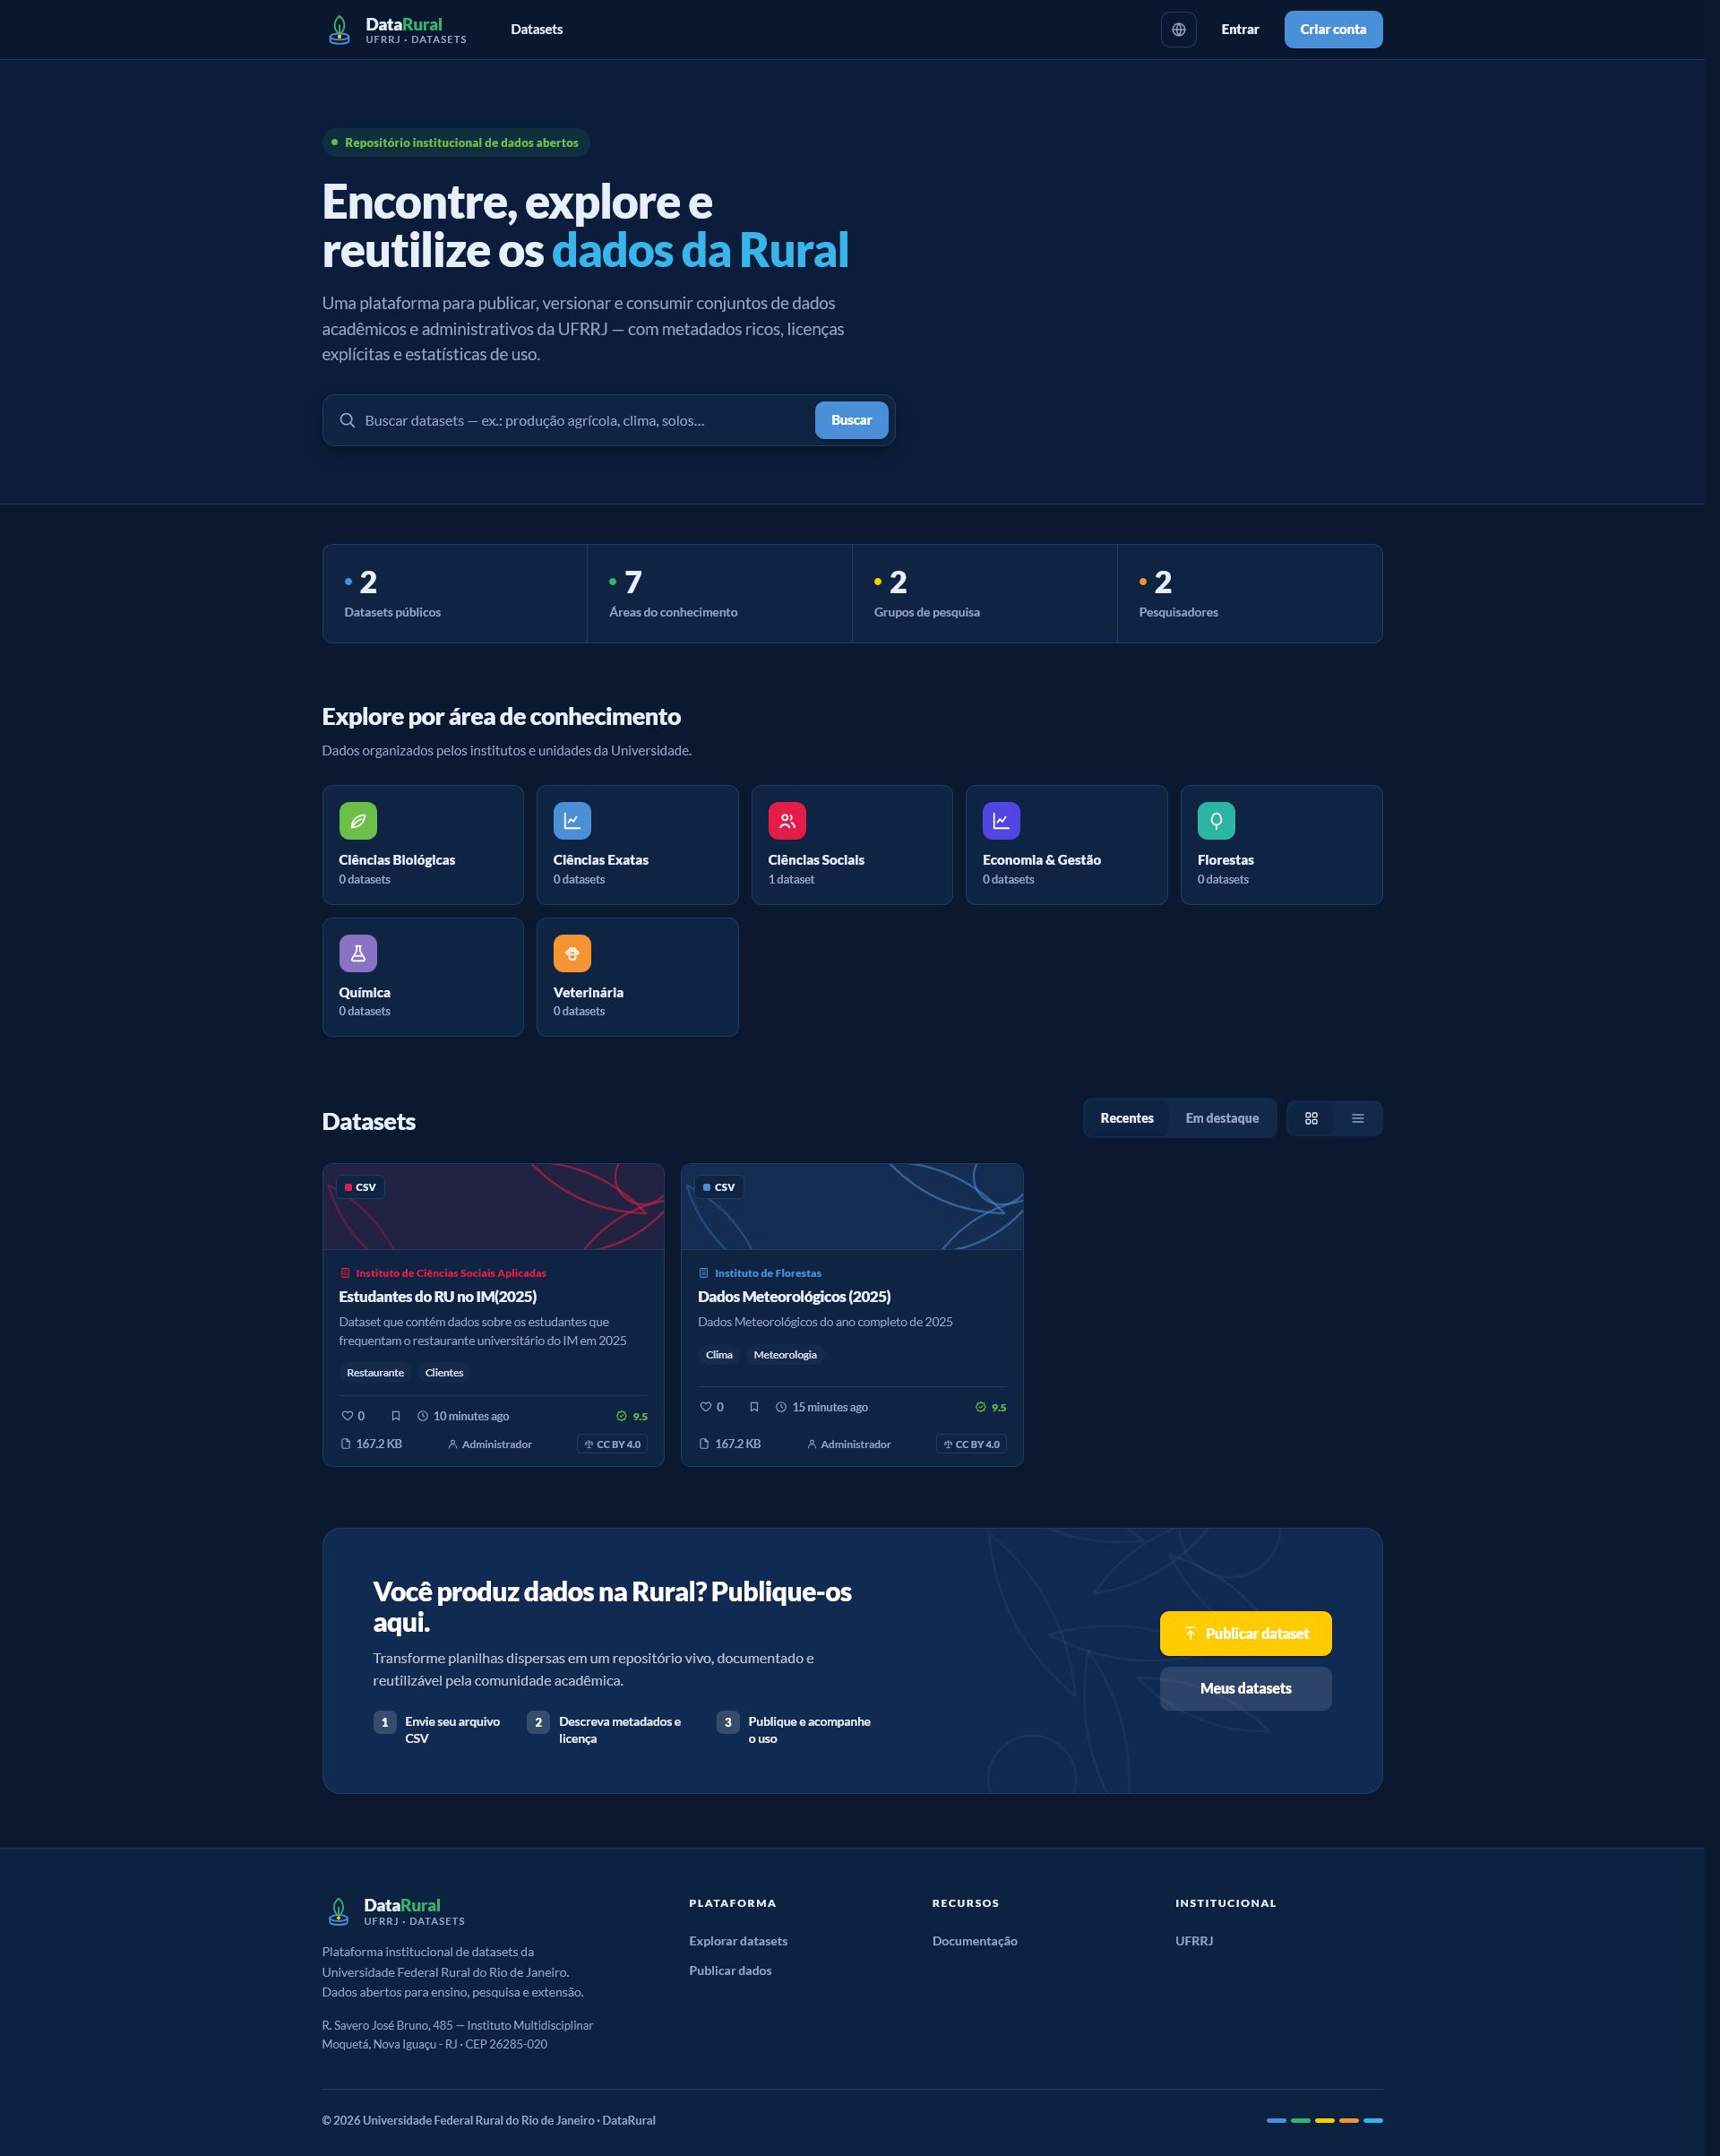
\includegraphics[width=0.85\textwidth,height=0.72\textheight,keepaspectratio]{imagens/pagina-inicial.png}
    \caption{Página inicial do DataRural, com busca de datasets públicos, indicadores do acervo e catálogo organizado por áreas de conhecimento da UFRRJ.}
    \label{fig:pagina_inicial}
    \centerline{\footnotesize Fonte: Elaborado pelos autores.}
\end{figure}
\FloatBarrier

O visitante pode utilizar a busca e a filtragem por área temática para localizar publicações e, em seguida, acessar a página de detalhes do conjunto escolhido. A consulta e o download de conteúdo público não exigem autenticação. Dessa forma, a separação entre navegação pública e operações de gerenciamento concretiza a distinção de acesso prevista na proposta: a identificação do usuário é exigida quando ele pretende publicar ou utilizar recursos pessoais, e não apenas para conhecer o acervo.

\subsection{Autenticação e controle de acesso}\label{sec:impl_acesso}

A tela de autenticação, apresentada na \reffigure{fig:tela_login}, oferece entrada por e-mail e senha, recuperação de acesso, encaminhamento para cadastro e a opção de acesso por conta Google. Após a autenticação, o usuário passa a acessar os recursos de publicação, grupos e favoritos. O acesso ao painel administrativo depende, adicionalmente, do papel global atribuído à conta.

\begin{figure}[!htbp]
    \centering
    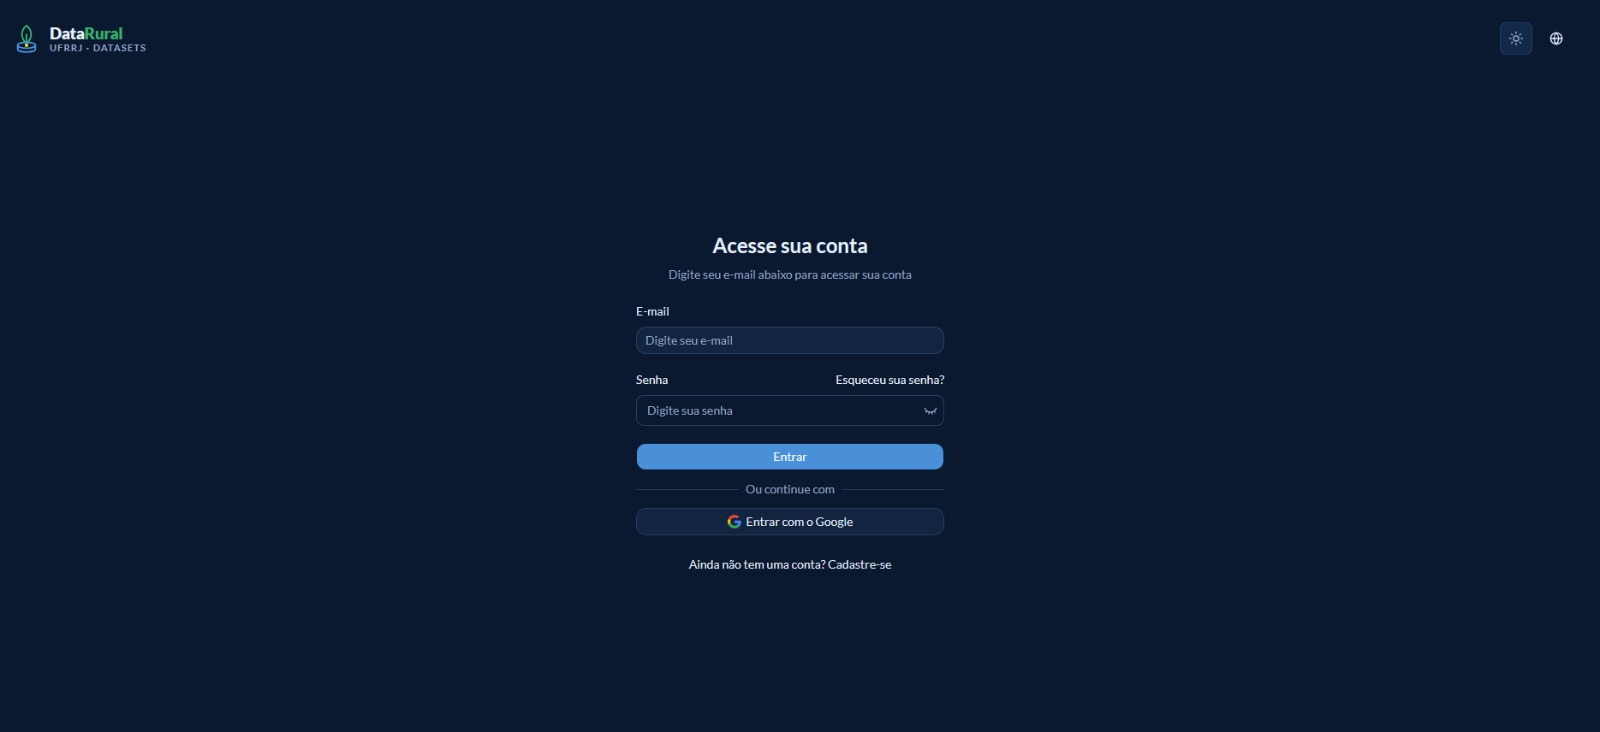
\includegraphics[width=0.65\textwidth]{imagens/login.jpeg}
    \caption{Tela de autenticação do DataRural, com acesso por e-mail e senha ou conta Google para utilização das funcionalidades restritas a usuários autenticados.}
    \label{fig:tela_login}
    \centerline{\footnotesize Fonte: Elaborado pelos autores.}
\end{figure}
\FloatBarrier

No servidor, a identidade autenticada é mantida por meio dos recursos de sessão do AdonisJS. O módulo Shield fornece proteção contra \textit{cross-site request forgery} (CSRF), complementando os mecanismos de autenticação. As rotas de publicação, gerenciamento de grupos, favoritos e administração aplicam \textit{middleware} de autenticação antes de executar as operações correspondentes.

A autorização considera também o recurso solicitado. Nos datasets individuais, a verificação utiliza a associação entre o conjunto e seu proprietário; nos datasets vinculados a grupos, considera a participação do usuário e o papel registrado em \textit{group\_members}. O papel global, associado ao campo \textit{role\_id} de \textit{users}, controla as operações administrativas. Essa separação implementa os dois níveis de permissão definidos na Seção~\ref{sec:controle_acesso}, evitando que a autenticação, isoladamente, seja suficiente para modificar qualquer publicação.

\subsection{Publicação de datasets}\label{sec:impl_publicacao}

A publicação é realizada por um assistente guiado de cinco etapas. O fluxo reúne a seleção dos arquivos, o preenchimento dos metadados, a descrição das colunas, a definição da licença e a revisão final. A divisão permite que o usuário confira separadamente o conteúdo enviado e as informações que contextualizam sua utilização.

Na primeira etapa, apresentada na \reffigure{fig:publicar_etapa1}, o usuário seleciona os arquivos CSV. A interface identifica o arquivo principal e oferece um controle para adicionar outros arquivos à mesma publicação. A captura mostra um arquivo com 1.000 linhas e 12 colunas, acompanhado de uma prévia das três primeiras linhas e dos tipos identificados. Também são apresentados indicadores de leitura do arquivo e uma estimativa de usabilidade, permitindo uma inspeção inicial antes do preenchimento dos metadados. O escopo adotado limita o envio ao formato CSV, com até 25~MB por arquivo.

\begin{figure}[!htbp]
    \centering
    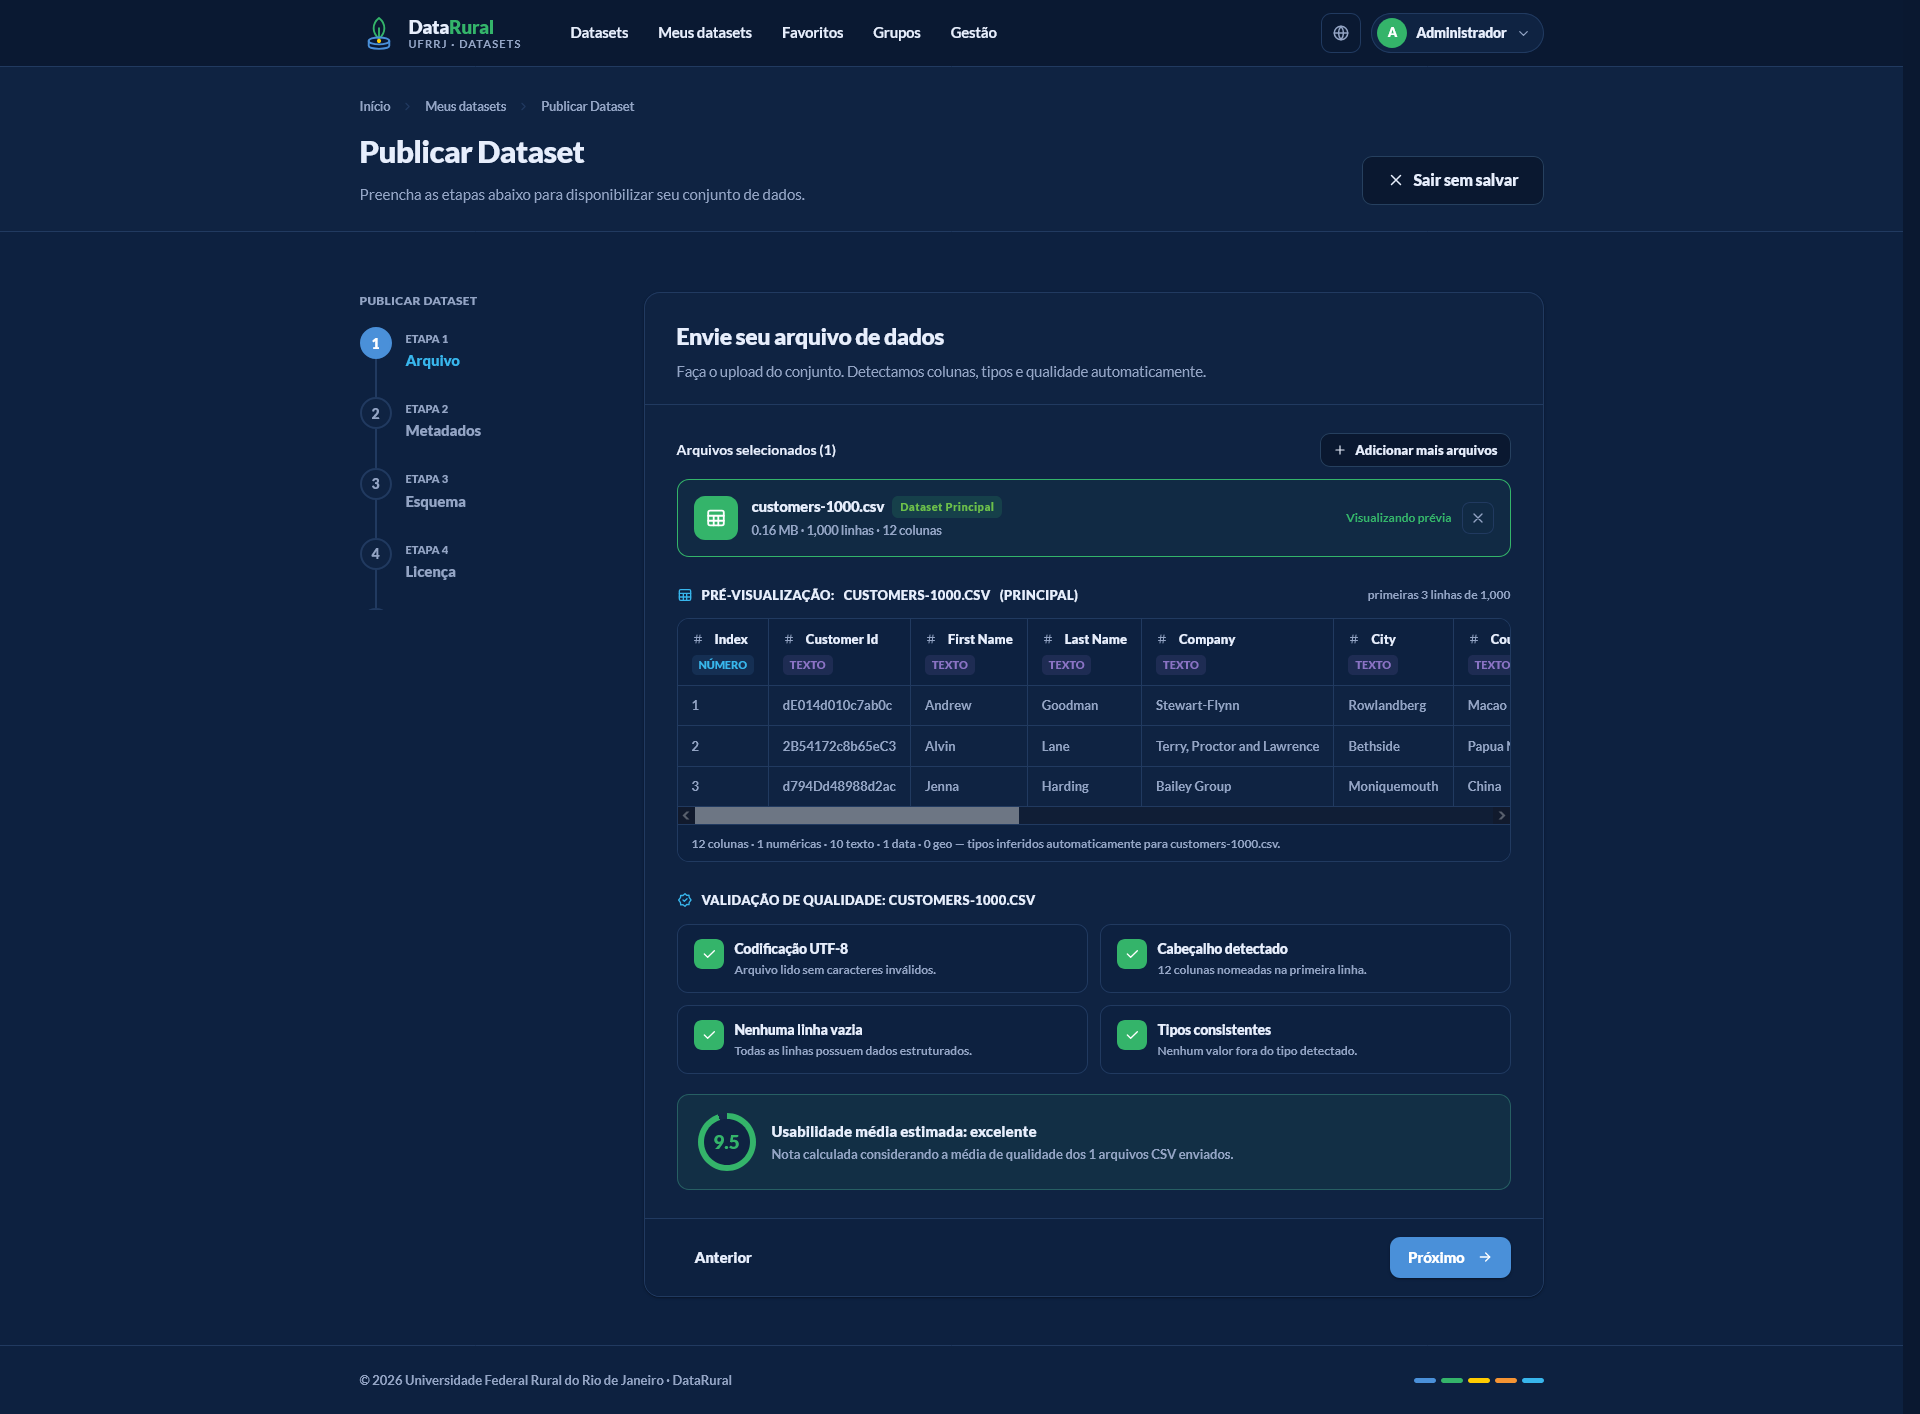
\includegraphics[width=0.85\textwidth,height=0.65\textheight,keepaspectratio]{imagens/publicar-dataset-01.png}
    \caption{Etapa 1 do assistente de publicação de datasets do DataRural: envio do arquivo CSV, identificação de sua estrutura e pré-visualização das primeiras linhas.}
    \label{fig:publicar_etapa1}
    \centerline{\footnotesize Fonte: Elaborado pelos autores.}
\end{figure}
\FloatBarrier

A segunda etapa, ilustrada na \reffigure{fig:publicar_etapa2}, reúne título, descrição, unidade ou instituto, área de conhecimento, período de cobertura, região e palavras-chave. Esses campos correspondem às informações descritivas da entidade \textit{datasets}. Seu preenchimento permite que a publicação seja identificada por características do conteúdo, e não apenas pelo nome do arquivo armazenado.

\begin{figure}[!htbp]
    \centering
    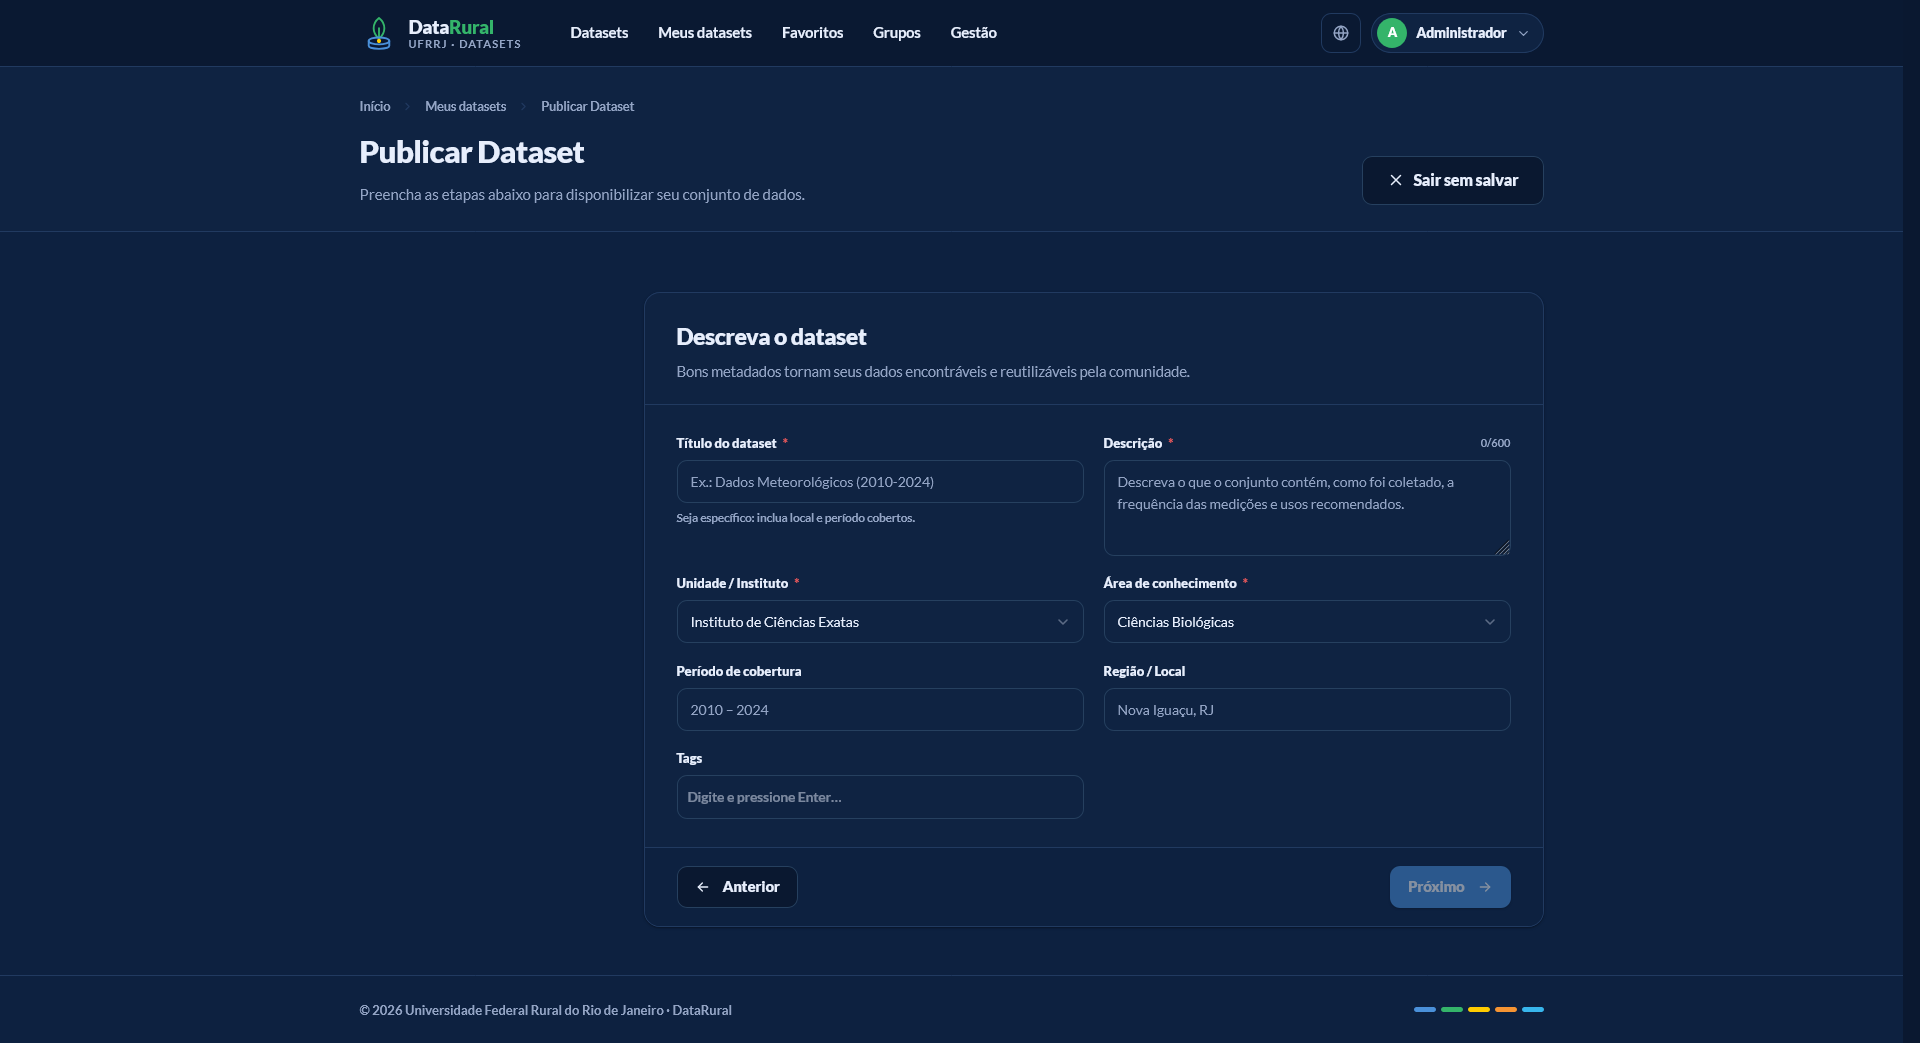
\includegraphics[width=0.85\textwidth,height=0.65\textheight,keepaspectratio]{imagens/publicar-dataset-02.png}
    \caption{Etapa 2 do assistente de publicação de datasets do DataRural: preenchimento dos metadados que descrevem o conjunto de dados, seu vínculo institucional e sua abrangência temporal e espacial.}
    \label{fig:publicar_etapa2}
    \centerline{\footnotesize Fonte: Elaborado pelos autores.}
\end{figure}
\FloatBarrier

Na terceira etapa, apresentada na \reffigure{fig:publicar_etapa3}, a interface lista as colunas do CSV e disponibiliza controles para revisão dos tipos e preenchimento das descrições. Esse dicionário de colunas complementa os metadados gerais: enquanto o título e a descrição contextualizam o conjunto, a documentação por coluna esclarece o significado de cada atributo. A revisão pelo responsável continua necessária, pois um tipo identificado automaticamente não determina, por si só, o significado científico da variável.

\begin{figure}[!htbp]
    \centering
    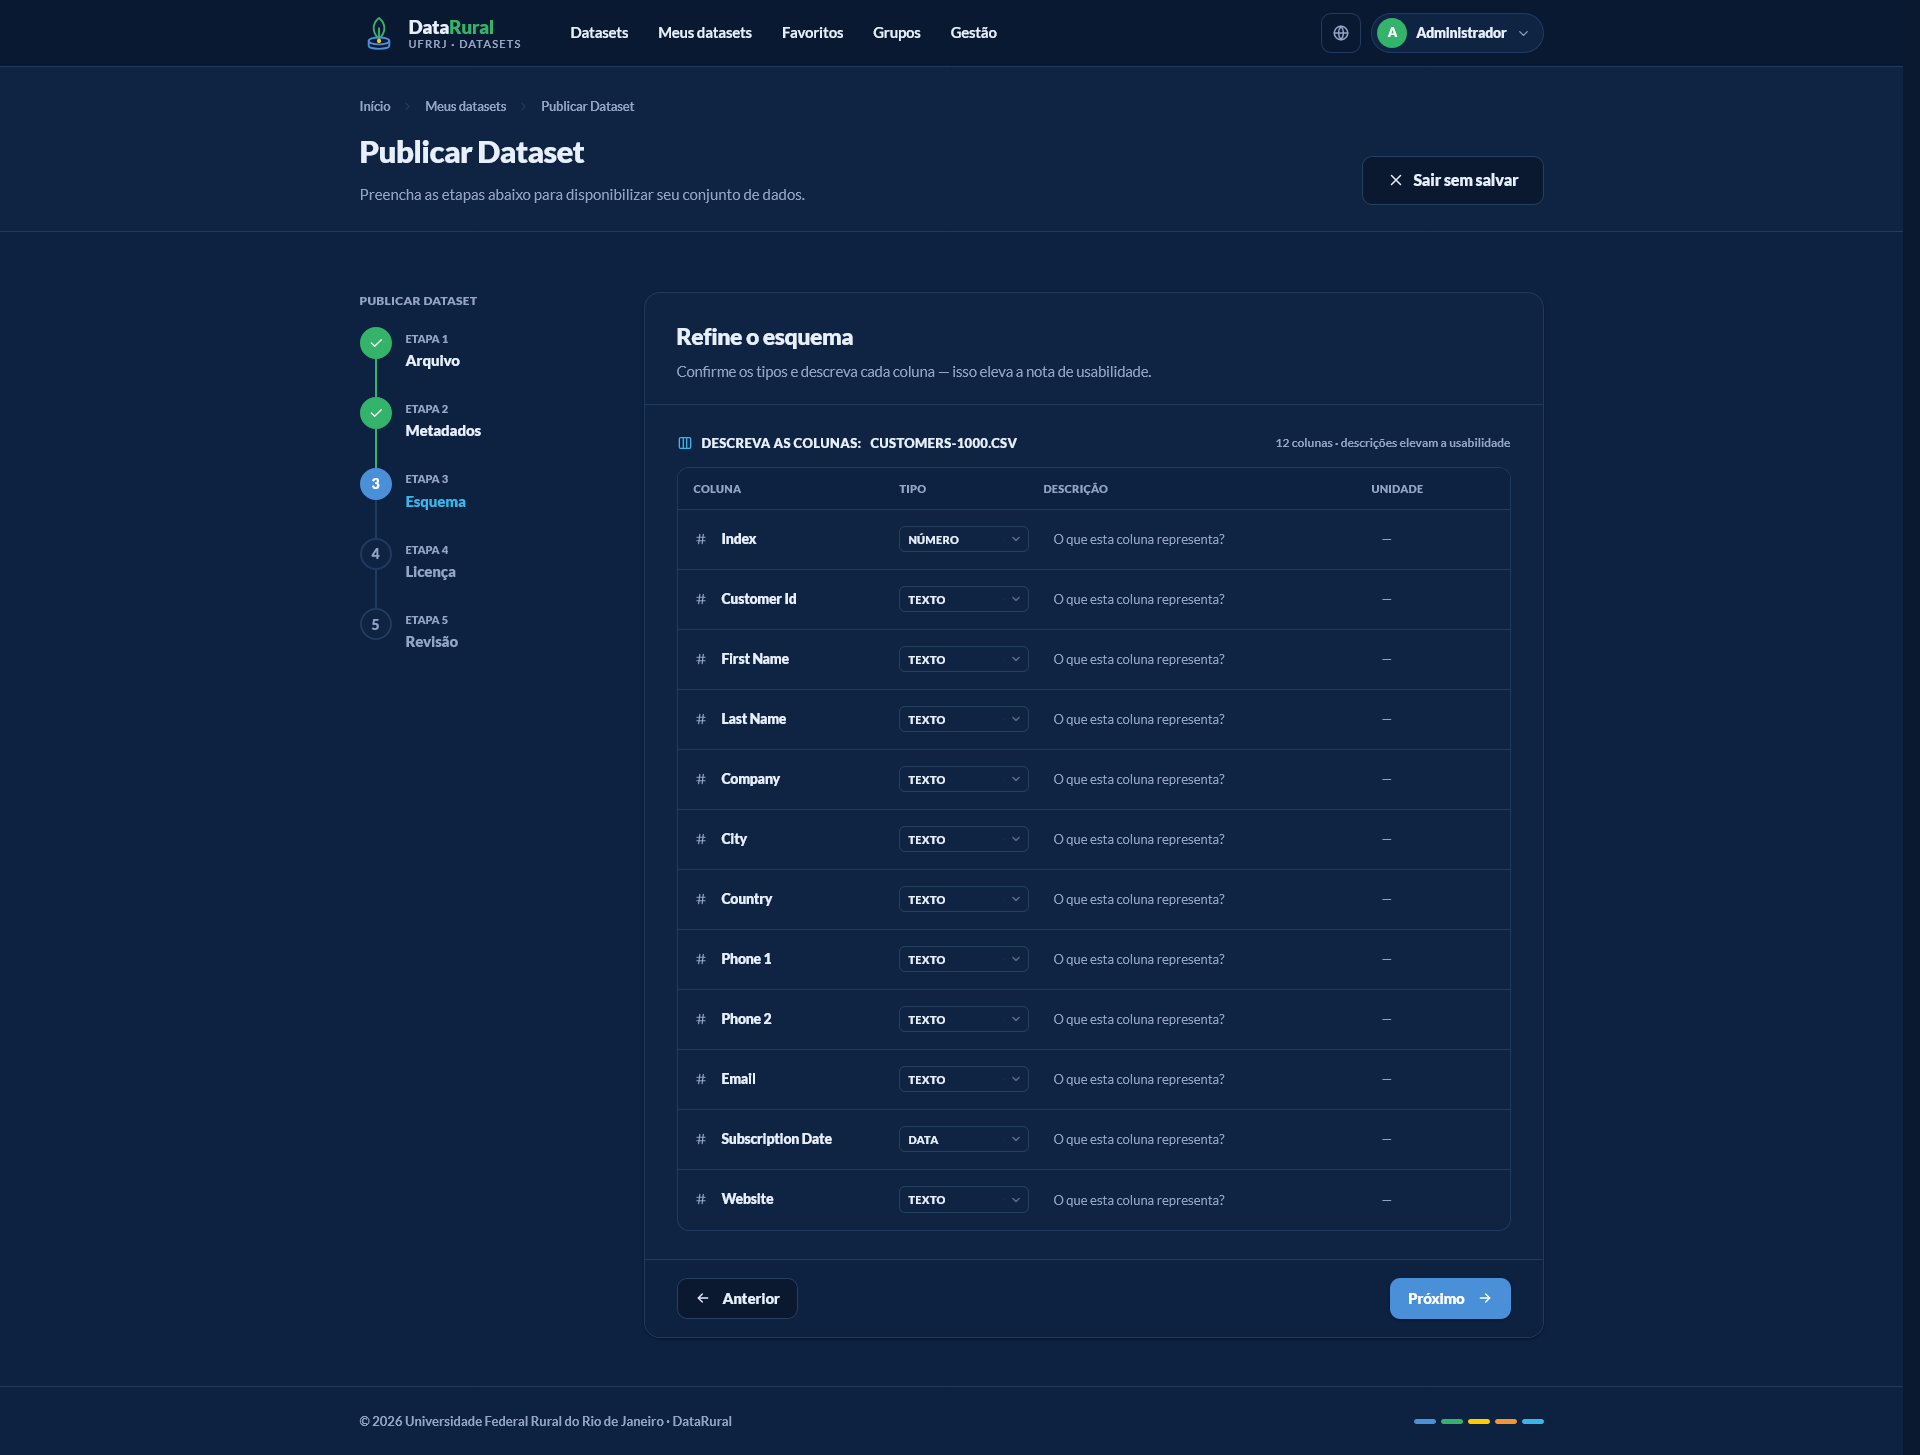
\includegraphics[width=0.85\textwidth,height=0.65\textheight,keepaspectratio]{imagens/publicar-dataset-03.png}
    \caption{Etapa 3 do assistente de publicação de datasets do DataRural: revisão dos tipos e preenchimento das descrições das colunas do CSV para compor o dicionário de dados.}
    \label{fig:publicar_etapa3}
    \centerline{\footnotesize Fonte: Elaborado pelos autores.}
\end{figure}
\FloatBarrier

A quarta etapa, ilustrada na \reffigure{fig:publicar_etapa4}, separa a escolha da licença da definição de visibilidade. A tela apresenta opções como CC BY 4.0, CC BY-SA 4.0, CC BY-NC 4.0, CC0 e ODbL, além de uma alternativa personalizada. A visibilidade determina se o conteúdo será público ou restrito; no controle de acesso descrito neste trabalho, os conjuntos privados são acessíveis ao proprietário ou aos membros autorizados do grupo associado. A seleção realizada nessa etapa é utilizada em conjunto com as verificações de autorização do servidor.

\begin{figure}[!htbp]
    \centering
    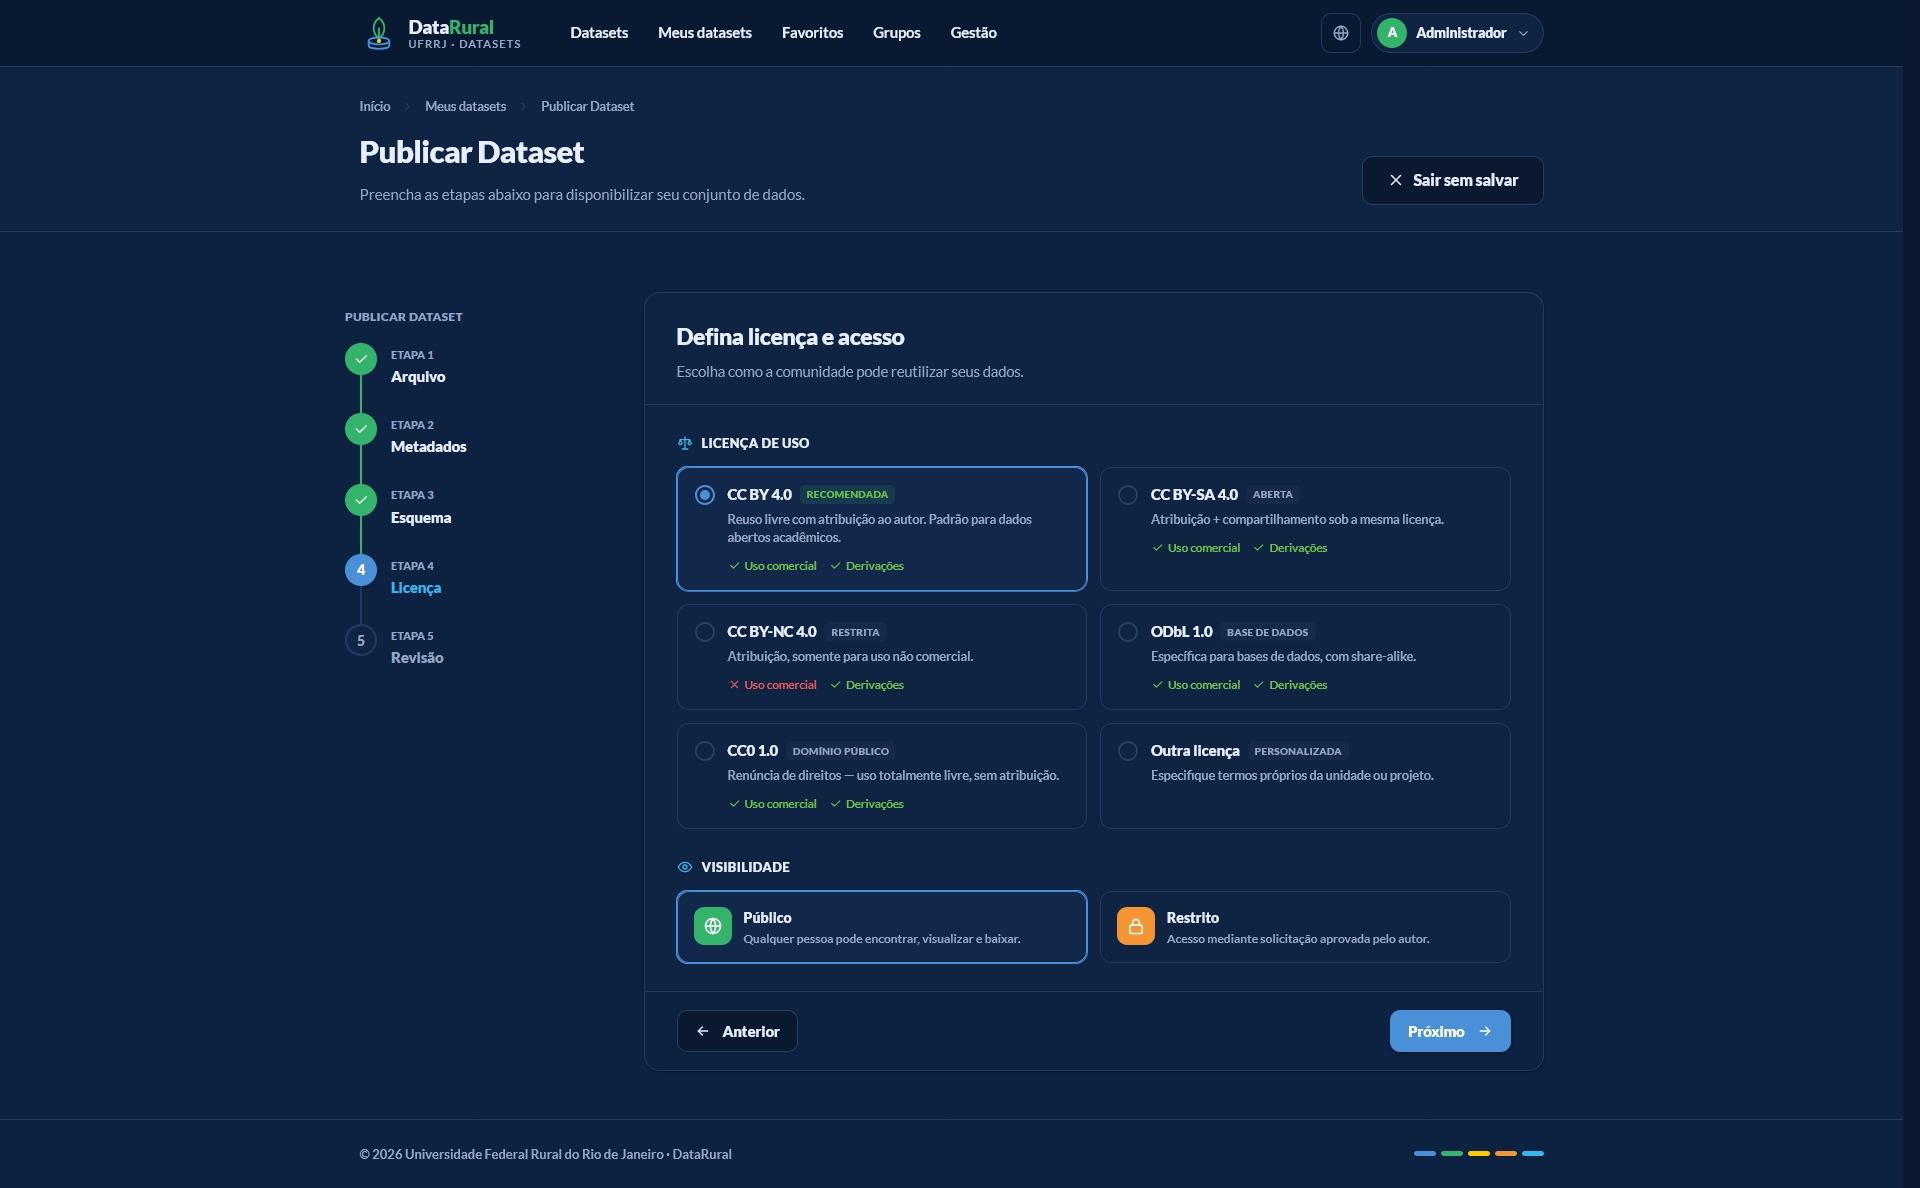
\includegraphics[width=0.85\textwidth,height=0.65\textheight,keepaspectratio]{imagens/publicar-dataset-04.png}
    \caption{Etapa 4 do assistente de publicação de datasets do DataRural: seleção da licença de uso e definição da visibilidade pública ou privada do conjunto de dados.}
    \label{fig:publicar_etapa4}
    \centerline{\footnotesize Fonte: Elaborado pelos autores.}
\end{figure}
\FloatBarrier

Na quinta etapa, apresentada na \reffigure{fig:publicar_etapa5}, o usuário confere um resumo do arquivo, dos metadados e das condições de uso e acesso. A interface oferece atalhos para revisar as informações e exige o aceite da declaração de conformidade antes da confirmação. Esse aceite registra a manifestação do responsável, mas não substitui a análise do conteúdo que ele pretende disponibilizar.

\begin{figure}[!htbp]
    \centering
    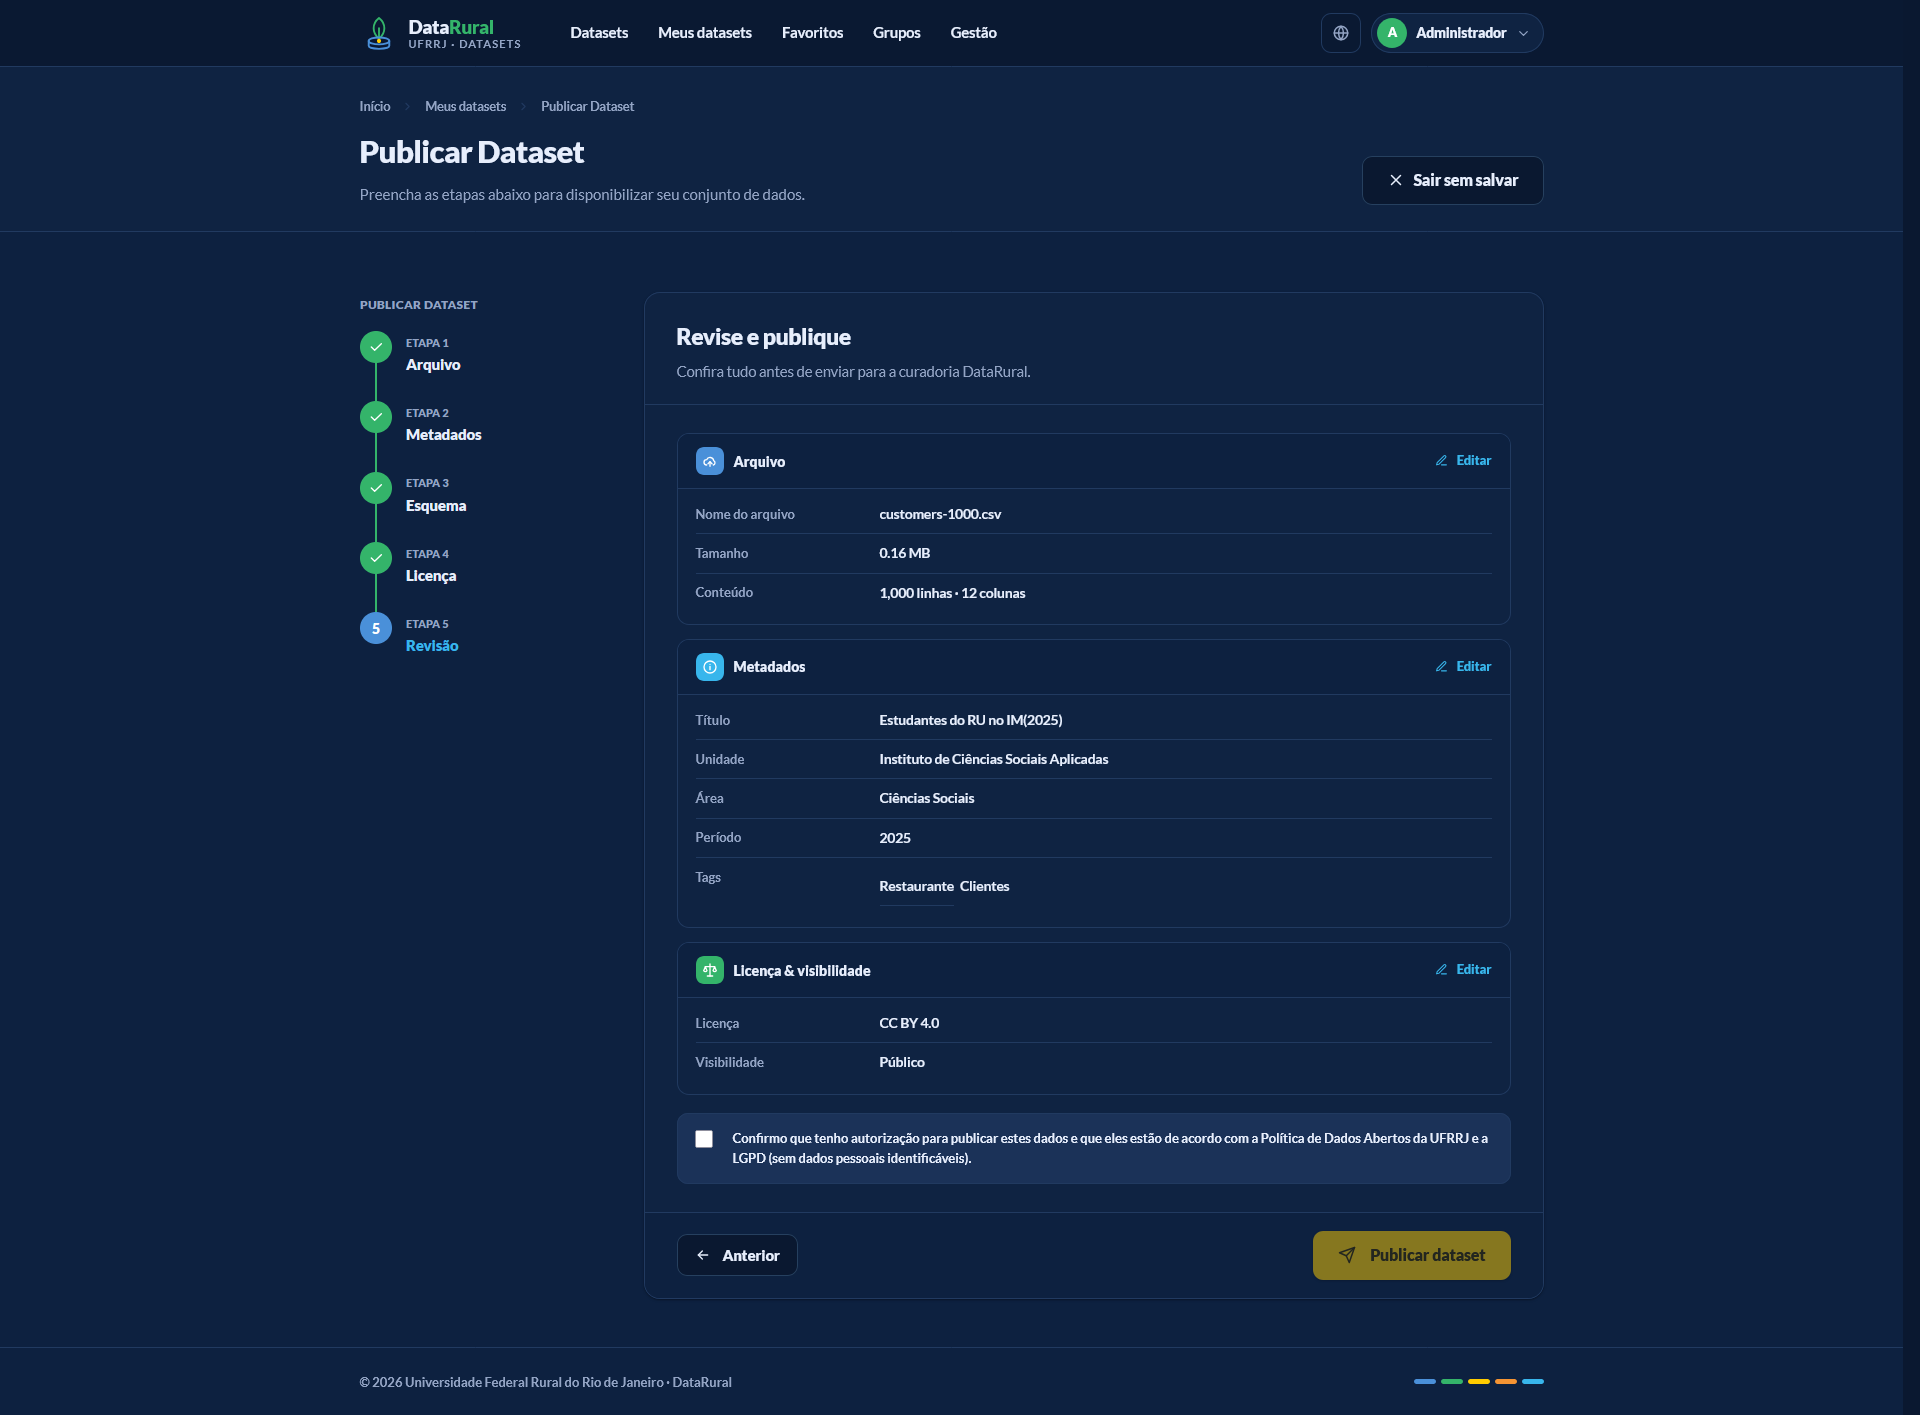
\includegraphics[width=0.85\textwidth,height=0.65\textheight,keepaspectratio]{imagens/publicar-dataset-05.png}
    \caption{Etapa 5 do assistente de publicação de datasets do DataRural: conferência das informações cadastradas e aceite da declaração de conformidade institucional antes de concluir a publicação.}
    \label{fig:publicar_etapa5}
    \centerline{\footnotesize Fonte: Elaborado pelos autores.}
\end{figure}
\FloatBarrier

A conclusão do fluxo associa os metadados da publicação ao usuário responsável e cria a versão inicial do dataset. Os registros de \textit{datasets}, \textit{dataset\_versions} e \textit{dataset\_version\_files} são criados em uma transação relacional, enquanto os anexos são mantidos no armazenamento de arquivos descrito anteriormente. Essa divisão distingue o registro institucional do conjunto, o estado de seus dados em uma versão e cada arquivo que compõe esse estado. O arquivo \texttt{README.md}, gerado para a versão, reúne as informações descritivas disponíveis no momento da publicação.

\subsection{Exploração e download dos dados}\label{sec:impl_exploracao}

Após selecionar um dataset, o usuário acessa a página de detalhes apresentada na \reffigure{fig:dataset_dashboard}. A interface reúne descrição, licença, informações sobre o arquivo e um dicionário de colunas. As abas separam a visão geral, o visualizador, a relação de arquivos e as versões, organizando em uma mesma página a consulta ao conteúdo e ao histórico da publicação.

\begin{figure}[!htbp]
    \centering
    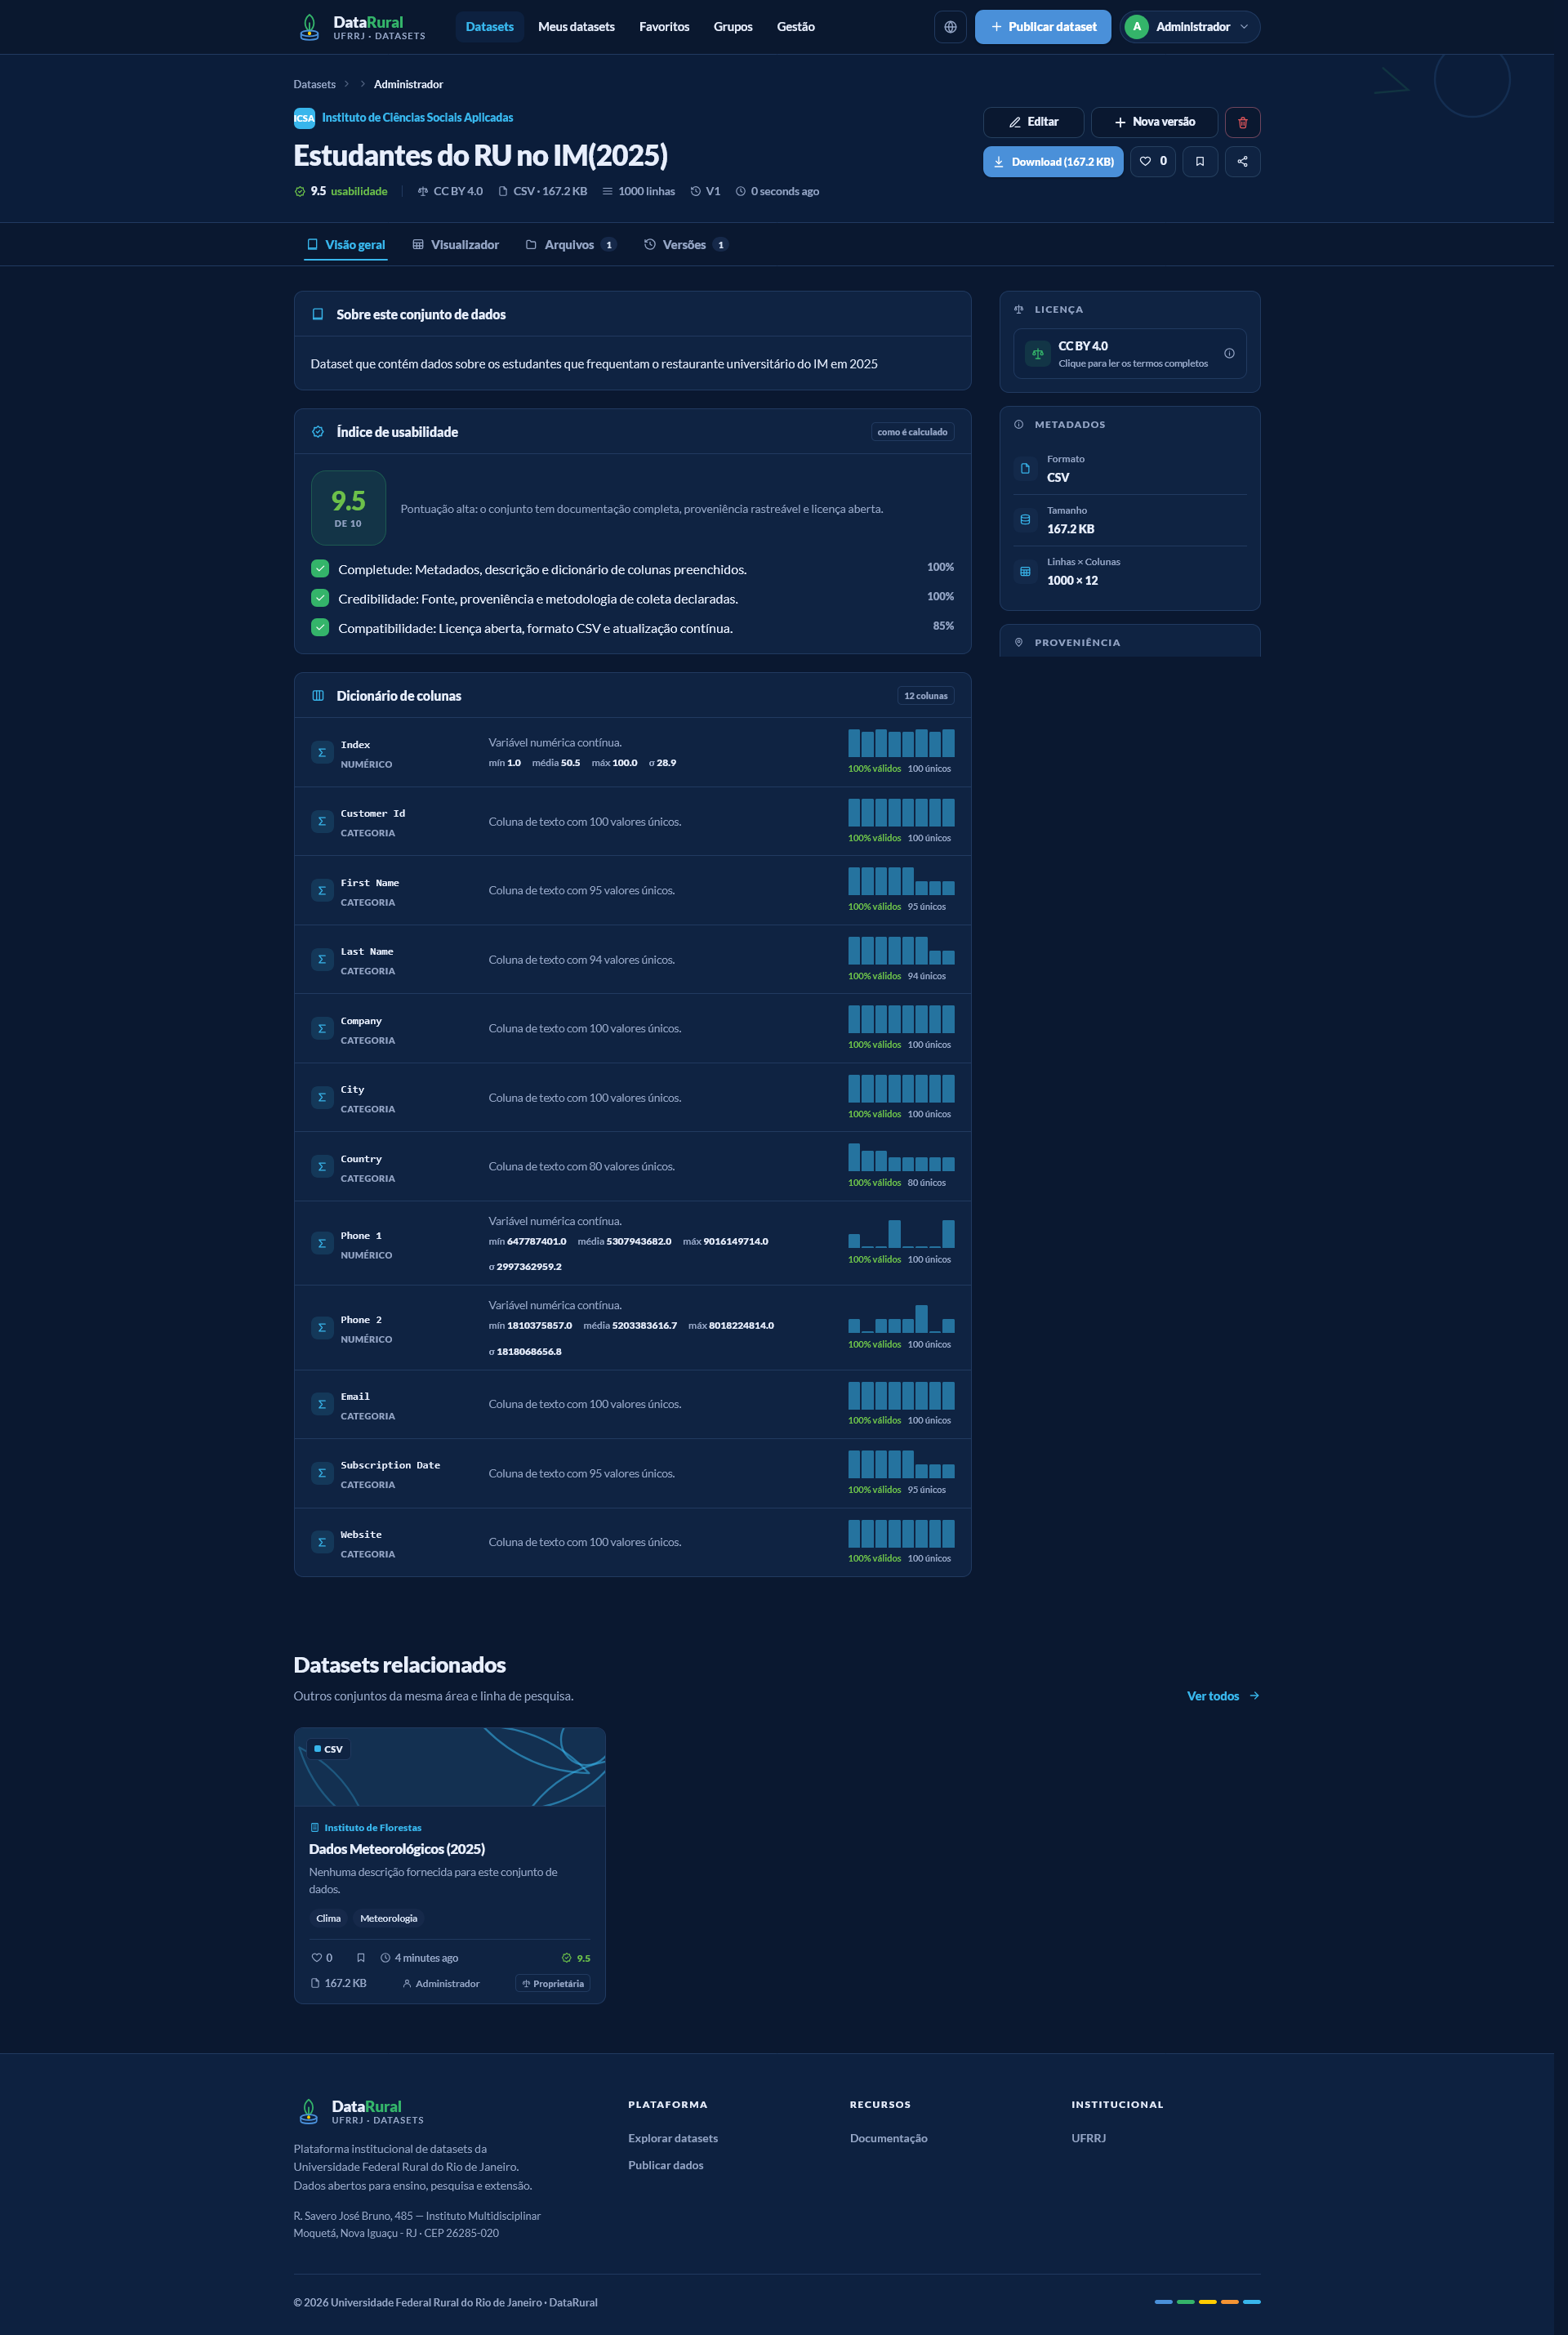
\includegraphics[width=0.85\textwidth,height=0.72\textheight,keepaspectratio]{imagens/dataset-detalhes-dashboard.png}
    \caption{Página de detalhes de um dataset no DataRural, com metadados, índice de usabilidade, dicionário de colunas e acesso às abas de visualização, arquivos e versões.}
    \label{fig:dataset_dashboard}
    \centerline{\footnotesize Fonte: Elaborado pelos autores.}
\end{figure}
\FloatBarrier

A visão geral apresenta o índice de usabilidade e informações resumidas por coluna. Esses elementos auxiliam a inspeção do material, mas não constituem uma validação da qualidade científica dos dados. Em particular, a pontuação exibida não deve ser interpretada como resultado de um teste de usabilidade da aplicação com participantes, pois sua finalidade é caracterizar aspectos da publicação.

A prévia tabular é processada no navegador: o componente interpreta o conteúdo do CSV e constrói a tabela de visualização. Assim, o usuário pode observar a estrutura e exemplos de valores antes de realizar o download. Essa funcionalidade não substitui ferramentas externas de análise e não corresponde à execução de consultas analíticas sobre o banco de dados da plataforma.

O download pode ser realizado por arquivo ou para todos os arquivos de uma versão, reunidos em um pacote ZIP. A disponibilização respeita a política de acesso do conjunto. Usuários autenticados podem também curtir a publicação ou adicioná-la aos favoritos. Essas ações são persistidas nas entidades \textit{dataset\_likes} e \textit{dataset\_favorites}, respectivamente, sem modificar a autoria ou a visibilidade do dataset. A separação permite distinguir uma interação pública de uma seleção pessoal de conjuntos para consulta posterior.

\subsection{Gestão pessoal de datasets}\label{sec:impl_gestao}

O painel \textit{Meus datasets}, apresentado na \reffigure{fig:meus_datasets}, concentra o acompanhamento das publicações pelo usuário autenticado. A tela apresenta indicadores de datasets publicados e curtidas, busca textual, seleção entre conjuntos pessoais e de grupos e categorias para publicações, rascunhos e conteúdos privados. A listagem organiza título, situação, curtidas e usabilidade de cada conjunto.

\begin{figure}[!htbp]
    \centering
    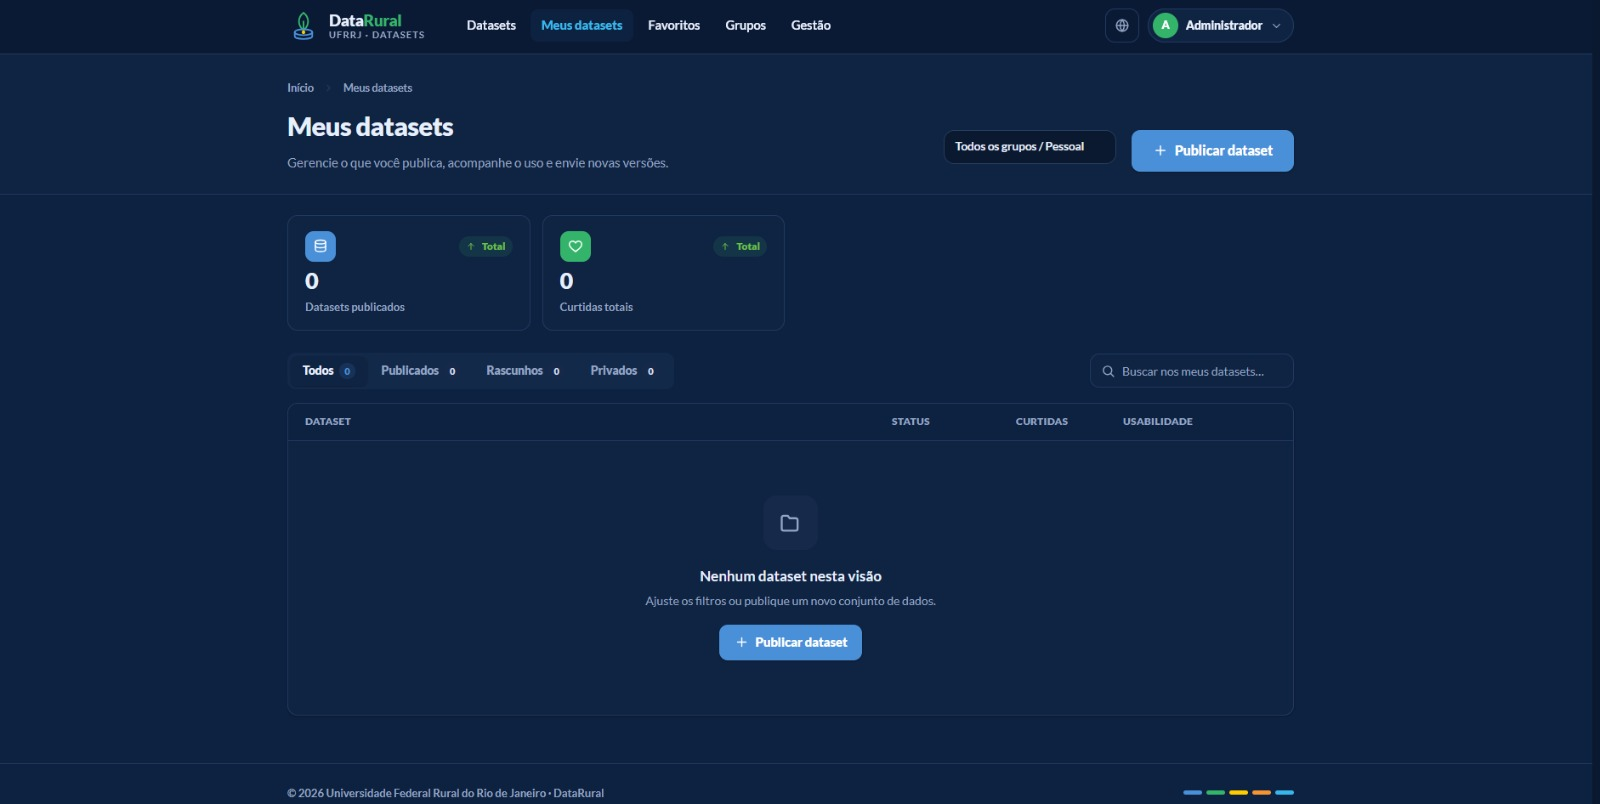
\includegraphics[width=0.85\textwidth]{imagens/meus-datasets.jpeg}
    \caption{Painel \textit{Meus datasets} do DataRural, com indicadores dos conjuntos de dados do usuário autenticado e controles de busca, filtragem e início de nova publicação.}
    \label{fig:meus_datasets}
    \centerline{\footnotesize Fonte: Elaborado pelos autores.}
\end{figure}
\FloatBarrier

A captura apresenta o estado vazio da listagem, com orientação para ajustar os filtros ou iniciar uma publicação. Esse estado também faz parte do fluxo de uso: antes de possuir conjuntos cadastrados, o usuário já encontra o caminho para criar seu primeiro dataset. Quando há publicações disponíveis, o painel funciona como ponto de acesso à consulta e à manutenção do acervo sob sua responsabilidade, enquanto as permissões continuam sendo verificadas pelo servidor.

\subsection{Versionamento e manutenção do histórico}\label{sec:impl_versionamento}

A atualização dos arquivos ocorre a partir de um dataset existente. Na página de detalhes, a ação de criação de uma nova versão permite enviar o conteúdo atualizado sem substituir o registro principal do conjunto. O usuário confirma o envio, e a versão subsequente permanece vinculada ao mesmo dataset. Na \reffigure{fig:dataset_dashboard}, o acesso à criação de versão aparece junto às ações de gerenciamento, enquanto uma aba específica organiza a consulta ao histórico.

A modelagem separa as responsabilidades dessa operação. A entidade \textit{datasets} mantém a identificação do conjunto; \textit{dataset\_versions} registra cada versão e sua associação ao dataset; e \textit{dataset\_version\_files} identifica os arquivos pertencentes a cada versão. Dessa forma, a inclusão de novos dados não exige criar outra publicação independente, e os arquivos anteriores mantêm sua vinculação ao histórico.

A exclusão de uma versão é lógica e utiliza o campo \textit{is\_deleted}. O registro deixa de aparecer como ativo nos fluxos comuns, mas permanece armazenado para possibilitar sua restauração. A manutenção do histórico preserva a possibilidade de recuperar uma versão anterior sem confundi-la com a mais recente. Tanto a criação de versões quanto as demais operações de manutenção dependem da autorização do proprietário ou do membro habilitado no grupo.

\subsection{Colaboração por grupos}\label{sec:impl_grupos}

A colaboração é implementada pelas entidades \textit{groups} e \textit{group\_members}. A primeira registra o grupo, sua finalidade e seu proprietário; a segunda associa cada participante ao grupo e mantém o papel que ele exerce naquele contexto. A vinculação de um dataset ao grupo é registrada em \textit{group\_id}, permitindo aplicar as permissões da equipe ao conjunto de dados.

Na utilização da plataforma, o responsável pode vincular um dataset a um grupo no qual possua permissão. A consulta e a manutenção desse conjunto passam então a considerar a participação e o papel de cada membro, conforme descrito na Seção~\ref{sec:impl_acesso}. Esse mecanismo permite compartilhar conjuntos privados sem torná-los públicos e sem atribuir a todos os participantes a condição de administrador da plataforma.

\subsection{Administração e auditoria}\label{sec:impl_auditoria}

O painel administrativo reúne a gestão de usuários e de áreas temáticas. Seu acesso é controlado pelo papel global da conta, distinguindo operações que afetam a organização da plataforma das atividades de publicação realizadas pelos usuários comuns. A manutenção das áreas temáticas, por exemplo, fornece as categorias utilizadas na classificação e na busca de datasets.

As alterações sobre entidades relevantes geram registros em \textit{audits}. Cada registro identifica a entidade alterada, o tipo de operação, os valores anteriores e posteriores, o usuário responsável e informações da requisição. A auditoria permite, portanto, acompanhar mudanças nos registros da aplicação, e não apenas nos arquivos enviados.

Versionamento e auditoria atendem a necessidades distintas de rastreabilidade. Uma edição da descrição pode gerar um evento de auditoria sem criar uma versão de arquivos; o envio de novos CSV, por sua vez, produz uma nova versão vinculada ao dataset. Essa distinção evita tratar toda alteração de metadados como uma atualização do conteúdo e permite acompanhar separadamente a evolução dos arquivos e as modificações nos registros que os descrevem.

\section{Síntese da implementação e atendimento à proposta}\label{sec:atendimento_proposta}

A implementação reúne publicação, consulta, manutenção de versões, colaboração e administração em uma mesma aplicação. A Tabela~\ref{tab:implementacao_requisitos} relaciona as funcionalidades descritas neste capítulo aos requisitos funcionais definidos na Tabela~\ref{tab:requisitos_funcionais}. Essa relação explicita como a proposta se traduz em operações e componentes do sistema, sem substituir a verificação sistemática de cada requisito por meio de testes.

\begin{longtable}{p{0.22\textwidth}p{0.18\textwidth}p{0.50\textwidth}}
\caption{Relação entre funcionalidades descritas na implementação do DataRural, requisitos funcionais da proposta e mecanismos utilizados para realizá-las.}\label{tab:implementacao_requisitos}\\
\toprule
\textbf{Funcionalidade} & \textbf{Requisitos} & \textbf{Implementação descrita} \\
\midrule
\endfirsthead
\toprule
\textbf{Funcionalidade} & \textbf{Requisitos} & \textbf{Implementação descrita} \\
\midrule
\endhead
Consulta ao catálogo & RF-17, RF-18 & Busca, filtragem por área e visualização prévia do CSV (Seções~\ref{sec:impl_catalogo} e~\ref{sec:impl_exploracao}). \\
Autenticação & RF-13 & Cadastro, entrada e manutenção da identidade por sessão, com proteção das rotas restritas (Seção~\ref{sec:impl_acesso}). \\
Publicação e documentação & RF-01, RF-02, RF-09, RF-10 & Assistente de envio de CSV, preenchimento de metadados e escolha de licença, associado aos registros do dataset e de sua versão inicial (Seção~\ref{sec:impl_publicacao}). \\
Controle de acesso e colaboração & RF-03, RF-04, RF-05, RF-19, RF-20 & Associação de datasets a grupos e verificação de propriedade, visibilidade e papéis para as operações de consulta e manutenção (Seções~\ref{sec:impl_acesso} e~\ref{sec:impl_grupos}). \\
Histórico de versões & RF-06, RF-07, RF-08 & Criação de versões vinculadas ao dataset, exclusão lógica e restauração (Seção~\ref{sec:impl_versionamento}). \\
Download e interações & RF-11, RF-12, RF-15, RF-16 & Download por arquivo ou em ZIP, com curtidas e favoritos registrados separadamente (Seção~\ref{sec:impl_exploracao}). \\
Administração e auditoria & RF-21, RF-22 & Gestão de usuários e áreas temáticas, com registros das alterações nas entidades relevantes (Seção~\ref{sec:impl_auditoria}). \\
\bottomrule
\end{longtable}

O escopo descrito utiliza CSV e armazenamento local de arquivos. A documentação das colunas, os indicadores da publicação e a prévia tabular apoiam a inspeção inicial, mas não substituem a análise científica do conteúdo nem constituem um ambiente completo de processamento de dados. A ampliação para outros formatos, a adoção de armazenamento de objetos e o consumo programático por uma API externa permanecem como possibilidades de continuidade.

As interfaces e os mecanismos apresentados demonstram a organização da solução desenvolvida, mas o trabalho não inclui uma avaliação sistemática com usuários da universidade. Também não são apresentados resultados de testes de carga ou uma avaliação abrangente de segurança. Assim, a descrição funcional não deve ser tomada como comprovação de desempenho, facilidade de uso ou prontidão para adoção institucional em larga escala. Essas limitações são retomadas no Capítulo~\ref{chp:CONCLUSAO}.
